
\begin{frame}{Knowledge Bases}
\begin{itemize}
\item Want to make the web smarter by \emph{understanding} the content \medskip
\item \emph{What} Entities? \emph{Which} Relations? \medskip
\item \emph{Encyclopedia that a Computer can understand} \medskip
 \item A standard reference set of entities, relations, type hierarchies \medskip
 \item \textbf{Wordnet}  The maiden knowledge base, has clean type system but limited entity base \medskip
 \item \textbf{Wikipedia} Huge, crowd sourced, but extremely loose and vague type systems \medskip
 \item Several knowledge bases have emerged as  middle ground 
\end{itemize}
\end{frame}

\begin{frame}{Freebase}
\begin{figure}[h]
 \centering
 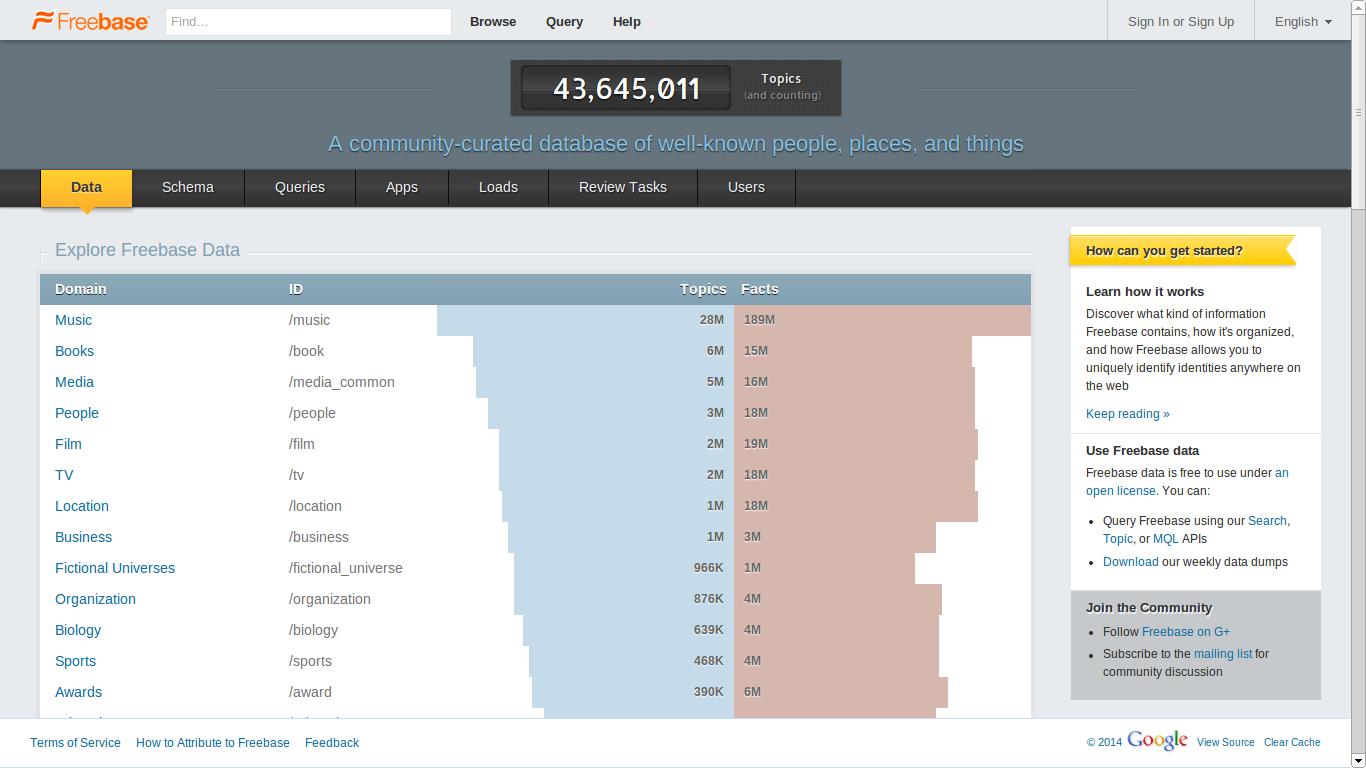
\includegraphics[bb=0 0 1366 768,scale=0.25]{./freebase.png}
 % freebase.png: 1366x768 pixel, 72dpi, 48.19x27.09 cm, bb=0 0 1366 768
\end{figure}
 
\end{frame}
\begin{frame}{Freebase}
\begin{itemize}
 \item Freebase relies on crowd sourcing for creation of a rich but clean knowledge base \medskip
 \item The development of Freebase follows the same chain as 
Wikipedia, with users flagging issues, and cleaning and augmenting information \medskip
\item Freebase also provides access to itself using web APIs.
\end{itemize}
\end{frame}

\begin{frame}{Knowledge Bases : Not there yet}
 \begin{itemize}
  \item \textcolor{red}{None} of the knowledge bases provides \textcolor{red}{entity priors} of any kind \medskip
  \item \textcolor{red}{Co-occurrence statistics} are also missing \medskip
  \item These pieces of information are really crucial for a number of tasks related like querying knowledge
  graphs. \medskip
  \item We motivate the need for such statistics after reviewing named entity disambiguation techniques. 
 \end{itemize}

\end{frame}

